\documentclass[sn-mathphys,pdflatex,iicol]{sn-jnl}% Math and Physical Sciences Reference Style

%%%% Standard Packages
\usepackage{polyglossia} % Must come before biblatex

\usepackage{bm}
\usepackage{csquotes}
\usepackage{fontspec}
\usepackage{hyperref}
%\usepackage{lua-visual-debug}
\usepackage{tabularx}
%%%%

\jyear{2022}

%% as per the requirement new theorem styles can be included as shown below
%%\theoremstyle{thmstyleone}%
%%\newtheorem{theorem}{Theorem}[section]% meant for sectionwise numbers
%% optional argument [theorem] produces theorem numbering sequence instead of independent numbers for Proposition
%%\newtheorem{proposition}[theorem]{Proposition}%
%%\newtheorem{proposition}{Proposition}% to get separate numbers for theorem and proposition etc.

%%\theoremstyle{thmstyletwo}%
%%\newtheorem{example}{Example}%
%%\newtheorem{remark}{Remark}%

%%\theoremstyle{thmstylethree}%
%%\newtheorem{definition}{Definition}%

\raggedbottom
%%\unnumbered% uncomment this for unnumbered level heads

\setdefaultlanguage{english}
\setotherlanguage{czech}

\hypersetup{
	pdfencoding=auto,
	unicode=true,
	bookmarksopen=true,
	bookmarksopenlevel=3
}

\newcommand{\name}[1]{\textit{#1}}
\newcommand{\mathfield}{\ensuremath{\mathbb}}
\newcommand{\mathmat}{\ensuremath{\mathbf}}
\newcommand{\mathset}{\ensuremath{\mathbb}}
\newcommand{\mathspace}{\ensuremath{\mathcal}}
\newcommand{\mathvec}{\ensuremath{\bm}}

\newcounter{enumroman}
\newenvironment{romanitems}{\begin{list}{\bfseries(\roman{enumroman})\hfill}{\usecounter{enumroman}\setlength{\labelwidth}{\leftmargin}\addtolength{\labelwidth}{-1\labelsep}\topsep=0mm plus 2pt\itemsep=0mm\parsep=0mm plus 2pt\itemindent=0mm}}{\end{list}}

\DeclareMathOperator*{\argmin}{arg\,min}
\DeclareMathOperator*{\argmax}{arg\,max}


\begin{document}

\copyrightyear{2022}
\copyrightclause{Use permitted under Creative Commons License Attribution 4.0 International (CC BY 4.0).}

\conference{Data and Model Quality for Mining and Learning with Graphs: Methods and Open Challenges
@ECML-PKDD 2022, September 23, 2022, Grenoble, France}

\title{Adaptive graph coarsening in the context of local graph quality}
\author[1,2]{Marek Dědič}[email=marek@dedic.eu,url=https://dedic.eu,orcid=0000-0003-1021-8428]
\cormark[1]
\author[2]{Lukáš Bajer}[email=lubajer@cisco.com,orcid=0000-0002-9402-6417]
\author[2]{Jakub Repický}[email=jrepicky@cisco.com,orcid=0000-0002-3695-1727]
\author[2]{Pavel Procházka}[email=paprocha@cisco.com]
\author[3]{Martin Holeňa}[email=martin@cs.cas.cz,url=http://cs.cas.cz/~martin,orcid=0000-0002-2536-9328]

\address[1]{Czech Technical University in Prague, Břehová 7, Prague, Czech Republic}
\address[2]{Cisco Systems, Inc., Karlovo náměstı́ 10, Prague, Czech Republic}
\address[3]{Institute of Computer Science, Czech Academy of Sciences, Pod vodárenskou věží 2, Prague, Czech Republic}

\cortext[1]{Corresponding author.}

\abstract{
Graph based models are used for tasks with increasing size and computational demands. We present a method for studying graph properties from the point of view of a downstream task. This method allows a user to precisely select the resolution at which the graph in question should be coarsened. Our method builds on an existing algorithm for pretraining on coarser graphs, HARP. We extend both main parts of the algorithm in order to observe the effect of graph coarsening to model quality on a fine level. We present a general framework for graph coarsenings, allowing is to cover, apart from HARP, two alternative algorithms based on graph diffusion convolution and evolutionary algorithms. Additionally, we present a novel way for refining the reduced graph in a targeted way based on the confidence of downstream classification for particular nodes. Together, these enhancements provide sufficient detail where needed, while collapsing structures where per-node information is not necessary for high model performance.
Hence, the method provides a general meta-model for enhancing graph embedding models such as node2vec. We apply it to several datasets, compare the considered coarsenings on them and discuss the differing behaviour on each of them in the context of their properties.
}

%%================================%%
%% Sample for structured abstract %%
%%================================%%

% \abstract{\textbf{Purpose:} The abstract serves both as a general introduction to the topic and as a brief, non-technical summary of the main results and their implications. The abstract must not include subheadings (unless expressly permitted in the journal's Instructions to Authors), equations or citations. As a guide the abstract should not exceed 200 words. Most journals do not set a hard limit however authors are advised to check the author instructions for the journal they are submitting to.
%
% \textbf{Methods:} The abstract serves both as a general introduction to the topic and as a brief, non-technical summary of the main results and their implications. The abstract must not include subheadings (unless expressly permitted in the journal's Instructions to Authors), equations or citations. As a guide the abstract should not exceed 200 words. Most journals do not set a hard limit however authors are advised to check the author instructions for the journal they are submitting to.
%
% \textbf{Results:} The abstract serves both as a general introduction to the topic and as a brief, non-technical summary of the main results and their implications. The abstract must not include subheadings (unless expressly permitted in the journal's Instructions to Authors), equations or citations. As a guide the abstract should not exceed 200 words. Most journals do not set a hard limit however authors are advised to check the author instructions for the journal they are submitting to.
%
% \textbf{Conclusion:} The abstract serves both as a general introduction to the topic and as a brief, non-technical summary of the main results and their implications. The abstract must not include subheadings (unless expressly permitted in the journal's Instructions to Authors), equations or citations. As a guide the abstract should not exceed 200 words. Most journals do not set a hard limit however authors are advised to check the author instructions for the journal they are submitting to.}

\keywords{
  Graph representation learning,
  Graph coarsening,
  Graph diffusion,
  Graph homophily,
  Performance-complexity trade-off,
  HARP
}


\maketitle

\section{Introduction}
Across a wide variety of applications and domains, graphs emerge as a domain-independent and ubiquitous way of organizing data. Consequently, machine learning on graphs has, in recent years, seen an explosion in popularity, breadth and depth of both research and applications. While there have been significant advances in algorithms for learning from graph data \cite{defferrard_convolutional_2016, kipf_semi-supervised_2017, li_deepergcn_2020}, the structure of the underlying data has, until recent works \cite{gasteiger_diffusion_2019, topping_understanding_2021, velickovic_geometric_2021, chamberlain_grand_2021}, received much less attention. In this work, we aim to take a closer look at the importance of the individual nodes and neighbourhoods that form a graph from the point of view of downstream tasks.

Typically, an application of machine learning to graphs has two phases: representation learning, which maps the graph into a Euclidean space, and a downstream task, such as classification, regression, or clustering. The first phase has very high computational demands, which can be substantially decreased with graph coarsening. However, it is known that there is an interplay between coarsening and the quality of embedding \cite{akyildiz_understanding_2020, makarov_survey_2021}, which in turn entails an interplay between coarsening and the quality of the downstream task.

Our work builds on the HARP \cite{chen_harp_2018} method for pretraining on coarsened graphs. In HARP, a graph is repeatedly coarsened and the coarser graphs are then used in reverse order (from coarsest to finest) to pre-train a graph representation learning algorithm. While HARP itself works with and modifies the graph structure, this is not the main interest of its authors, who focus more on the obtained representation of the original graph. In our work, we aim to leverage such a graph coarsening approach to study the properties of graphs and graph embedding models from the point of view of the graph structures getting coarsened with the additional benefit of decreasing computational requirements. We modify and generalize the HARP framework to closely study the relationship between graph coarsenings and graph quality in terms of the performance of a downstream task. In our case, we chose transductive node classification as the ultimate task, however, the presented algorithms are general graph representation learners that can be utilized for a wide variety of tasks.

\todo[inline]{Relation to ITAT paper?}

The main contributions of this work are the general framework for graph coarsening and extensions of the HARP algorithm. We extend both main parts of the algorithm in order to observe the effect of graph coarsening to model quality on a fine level. We present two alternative graph coarsening schemes based on graph diffusion convolution and evolutionary algorithms. Additionally, we present a novel way for un-coarsening the reduced graph in a targeted way based on the confidence of downstream classification for particular nodes.

In the next section, related work and its relationship to this work are discussed. Following that, in Section \ref{sec:harp-framework}, HARP, the method our work builds on, is presented, together with our extension of it into a general framework for graph coarsening. Section \ref{sec:our-method} is the core of this work, presenting first our extension of the prolongation step, as well as our proposed alternative graph coarsening schemes. Finally, these proposals are experimentally verified and compared in Section \ref{sec:experimental-evaluation}.

\section{Related work}

The publications most relevant to our research are \cite{chen_harp_2018}, in which the HARP approach is proposed, and \cite{gasteiger_diffusion_2019}, in which graph coarsening is performed by means of graph diffusion. Because we directly extend, modify or combine those methods, they will be explained in detail in Sections \ref{sec:harp} and \ref{sec:gdc-coarsening}. Other important works concerning graph coarsening are \cite{akyildiz_understanding_2020, chen_graph_2022}, which survey numerous coarsening methods, \cite{huang_scaling_2021}, which presents results concerning scalability or graph coarsening, and \cite{loukas_graph_2019} which shows relationships of graph coarsening to properties of the Laplacian. In view of the fact that the HARP approach, which we extend and modify, is a multilevel approach, we paid attention also to the multilevel graph coarsening methods proposed in \cite{xie_graph_2020} and \cite{zhang_harp_2021}, the latter being also inspired by HARP.

In a broader context, our research is related to the more general topic of graph reduction, which apart from graph coarsening includes also graph sparsification. A general framework covering both coarsening and sparsification has been proposed in \cite{bravo_hermsdorff_unifying_2019}. Elaboration of graph coarsening methods in machine learning can built on several decades of succesful application of their main kinds, such as pairwise aggregation, independent sets, or algebraic distance, in numerical linear algebra \cite{chen_graph_2022}.

\section{The HARP framework}

In this Section, firstly, a brief overview of the HARP framework for graph coarsening \cite{chen_harp_2018} is presented, followed by our analysis of the properties of graph coarsenings in general.

\subsection{HARP}
\todo[inline]{Explanation of the general structure of HARP, without going into detail about the coarsening procedure}
HARP is a method for improving the performance of graph representation learning (i.e. graph embedding) algorithms such as DeepWalk \cite{perozzi_deepwalk_2014}, LINE \cite{tang_line_2015}, PTE \cite{tang_pte_2015} or node2vec \cite{grover_node2vec_2016}. The method is a combination of dataset augmentation and pre-training based on the general principle that graph-based models train more efficiently on smaller graphs and can thus be pre-trained on a coarsened representation of the graph at hand. Moreover, the coarsened graphs approximate the global properties of the original data, enabling the representations to better encapsulate such a global structure. In an overview, the method consists of the following steps:

Consider an undirected graph \( G \) with nodes \( V \left( G \right) \) and edges \( E \left( G \right) \). The aim of the graph coarsening part of the algorithm is to generate a sequence of graphs \( G_0, G_1, G_2, \dots, G_L \) where \( G_0 = G \) and \( L \in \mathfield{N} \) is a hyper-parameter of the method. In this sequence, each graph \( G_i \) is generated from the graph \( G_{i - 1} \) by coarsening it -- lowering the number of nodes and edges while preserving the general structure of the graph. Following \cite{chen_harp_2018}, let \( \psi_i \) denote the mapping between the graphs such that \( V \left( G_i \right) = \psi_i \left( V \left( G_{i - 1} \right) \right) \).

\begin{itemize}
  \item \textbf{Dataset augmentation}. The graph \( G \) is consecutively reduced in size by the application of several graph coarsening schemas. In each step, the coarsened graph can be viewed as an ever coarser representation of the graph data and its global structure. This step can be run ahead-of-time to produce the resulting coarsened graphs \( G_0, G_1, \dots, G_L \).
\end{itemize}
After all the coarsened graphs are pre-computed, the method itself can be executed by repeating the following steps on the graphs from the coarsest to the finest (i.e. from \( G_L \) to \( G_0 \)):
\begin{itemize}
  \item \textbf{Training on an intermediary graph}. The graph embedding model is trained on \( G_i \), producing \( \Phi_{G_i} \), an embedding of the graph in a Euclidean space.
  \item \textbf{Embedding prolongation}. The embedding \( \Phi_{G_i} \) is prolonged from the current graph to one that is one step closer to \( G_0 \), yielding \( \Phi_{G_{i - 1}} \). This embedding is used as the starting state for the graph model which is to be trained on \( G_{i - 1} \).
\end{itemize}
These steps are repeated until \( \Phi_{G_0} \) is computed. While the training step of this schema is a straightforward application of one of the aforementioned embedding algorithms to \( G_i \), the particular details of the coarsening and prolongation steps are further explained in Sections \ref{sec:adaptive-prolongation} and \ref{sec:harp-coarsening}.

The first step is independent of the rest of the computation and can be done ahead of time. The last two steps can be seen as a form of pre-training for the model that is to be learnt on the original graph. The whole HARP pipeline is demonstrated in Figure \ref{fig:harp-overview}.\todo{The image isn't exactly correct}

\begin{figure}
  \centering
  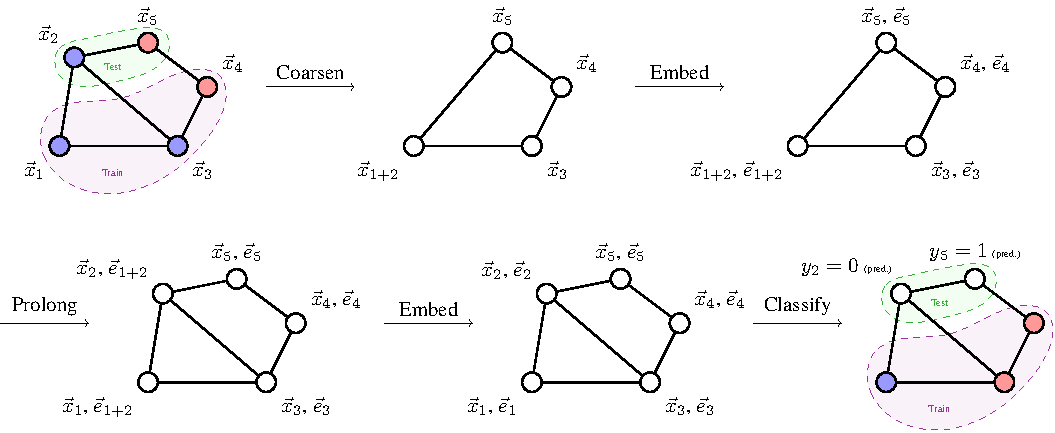
\includegraphics[width=\linewidth]{images/harp-overview/harp-overview.pdf}
  \caption{An overview of the HARP processing pipeline with one level of coarsening}
  \label{fig:harp-overview}
\end{figure}

\subsection{Properties of graph coarsenings}

The HARP framework presents a particular way of producing coarsened graphs. In general, however, we would like to describe any coarsening of a graph in order to be able to explore the set of all coarsened graphs to study the properties of both the applied algorithms, as well as the underlying data.

To properly describe the set of all coarsening, dome assumptions need to be made about what constitutes a coarsening. In our work, we define a coarsening as a set \( \mathcal{C} \subseteq E \left( G \right) \), that is a subset of edges of the original graphs. The graph \( H = \varphi_\mathcal{C} \left( G \right) \) obtained by applying this coarsening to \( G \) is obtained from \( G \) by contracting all edges in \( \mathcal{C} \)\footnote{Whether to allow parallel edges to arise from this operation is left to the user, in our work, we didn't.}. This description of a graph coarsening is inspired and builds upon the work \cite{schulz_mining_2019} with the relation between these two approaches further described in Appendix \ref{apdx:coarsening-as-pihom}.

\section{HARP extension for flexible performance-complexity balancing}

Graph-based methods such as node2vec typically have a large number of parameters -- on the widely used OGBN-ArXiv dataset (see \cite{hu_open_2021}), the state-of-the-art node2vec model has over 21 million parameters. At the same time, recent works in the domain of graph learning have started to focus more heavily on simpler methods as a competitive alternative to heavy-weight ones (see \cite{frasca_sign_2020,huang_combining_2020,salha_keep_2019,zhang_eigen-gnn_2021}). As the authors of \cite{chen_harp_2018} observed, HARP improves the performance of models when fewer labelled data are available. The proposed lower complexity models based on HARP could also improve performance in a setting where only low fidelity data are available for large parts of the graph. Coarser models could be trained on them, with a subsequent training of finer models using only a limited sample of high fidelity data.

In this work, we extend the general HARP framework to study the preformance-complexity characteristics of graph data. To this end, we propose alternatives to both the coarsening as well as the prolongation step of HARP. First, in Section \ref{sec:adaptive-prolongation}, we replace the simple prolongation approach by an adaptive prolongation algorithm. Second, in Section \ref{sec:coarsening-algorithms}, we study two alternative ways of coarsening the graph.

\subsection{The adaptive prolongation approach}\label{sec:adaptive-prolongation}

In standard HARP, once the coarsened graphs are obtained, the way to train the graph embedding is fairly straightforward. Starting with the coarsest graph, an embedding model such as node2vec is trained for a given amount of training epochs. Following that, a step to a graph that is one level finer is made. The embedding learned on the immediately preceding coarser graph is \name{prolonged} to the embedding of the following finer graph, in which the representations of merged nodes are copied and reused. Then, with this prolonged embedding as the starting state, the embedding algorithm continues training and this process is repeated until reaching the original graph.

While this style of prolongation is fine when HARP is used only as a means of pre-training, this approach is far too crude when studying the relationship between graph complexity and the quality of graph embedding and subsequent downstream applications. For example, the widely-used Cora dataset \cite{yang_revisiting_2016} has in its original form 2708 nodes, while the graph resulting from one application of the HARP coarsening schema has only about 1100 nodes (exact numbers may differ run-by-run). Such a relatively high reduction ratio effectively prevents any sufficient understanding of the relationship between graph reduction and changes in the quality of its embedding.

In order to offer a more fine-grained observation of the graph complexity and its effect on the downstream task, we present the adaptive prolongation approach. This algorithm works with the pre-coarsened graphs produced for example by HARP, however, the embedding is learned in a different manner.

\begin{algorithm}
  \caption{Adaptive prolongation}
  \label{alg:adaptive-prolongation}
  \begin{algorithmic}
    \Require $ G $ \Comment The original graph
    \Require $ \mathvec{e}_{i+1} $ \Comment The previous embedding
    \Require $ \mathvec{y}_\mathrm{train} $ \Comment Training labels
    \Require $ replacement\_maps $ \Comment A list of records of all the original graph coarsenings
    \Require $ n_p $ \Comment The number of nodes to prolong
    \Ensure $ merges\_to\_prolong $ \Comment A list of node merges to be prolonged (\enquote{undone})
    \Ensure $ new\_replacement\_maps $ \Comment Updated coarsening records without the prolonged merges
    \Statex
    \State $ node\_order = \Call{get\_node\_order}{G, \bm{e}_{i+1}, \bm{y}_\mathrm{train}, replacement\_maps} $
    \State $ merges\_to\_prolong \gets \Call{select\_nodes}{node\_order, n_p, replacement\_maps} $
    \State $ new\_replacement\_maps \gets \Call{undo\_merges}{replacement\_maps, merges\_to\_prolong} $
    \Statex
    \Function{get\_node\_order}{$ G, \bm{e}_{i+1}, \bm{y}_\mathrm{train}, replacement\_maps $}
        \State $ \bm{e}_0^\mathrm{temp} \gets \Call{fully\_prolong\_embedding}{\bm{e}_{i+1}, replacement\_maps} $
        \State $ model \gets \Call{train\_downstream\_model}{\bm{e}_0^\mathrm{temp}, \bm{y}_\mathrm{train}} $
        \State $ entropy\_per\_node \gets H \left( \Call{predict}{model, node} \right) $ for each $ node \in V \left( G \right) $
        \State \Return $ V \left( G \right) $, sorted in descending order by $ entropy\_per\_node $
    \EndFunction
    \Statex
    \Function{select\_nodes}{$ ordered\_nodes, n_p, replacement\_maps $}
        \State $ selected\_merges \gets \left\{ \right\} $
        \For{$ node \in ordered\_nodes $, until $ \left\lvert selected\_merges \right\rvert = n_p $}
            \State $ merge \gets \Call{resolve\_merge}{node, selected\_merges, replacement\_maps} $
            \State If $ merge \neq \mathrm{null} $, add $ merge $ to $ selected\_merges $
        \EndFor
        \State \Return $ selected\_merges $
    \EndFunction
    \Statex
    \Function{resolve\_merge}{$ node, already\_selected\_merges, replacement\_maps $}
        \State $ merge \gets \mathrm{null} $
        \For{$ replacement\_map \in replacement\_maps $ from finest graph to coarsest}
            \State $ merge\_candidate \gets $ find in $ replacement\_map $ a merge that affects $ node $, continue with next $ replacement\_map $ if not found
            \If{$ merge\_candidate \in already\_selected\_merges $}
                \State \Return $ merge $
            \EndIf
            \State $ merge \gets merge\_candidate $
            \State Apply $ merge $ to $ node $, so that in the next loop, a subsequent merge may be selected
        \EndFor
        \State \Return $ merge $
    \EndFunction
  \end{algorithmic}
\end{algorithm}

The adaptive prolongation approach (Algorithm \ref{alg:adaptive-prolongation}) uses the pre-computed coarsened graphs as a way to progressively increase the number of nodes with which the embedding is trained. However, its iterations of embedding training and prolongation are decoupled from the pre-computed coarsened graphs. Instead, in each step of the training, the current embedding is used to train a node classifier that guides which nodes should be prolonged. The node classifier is equivalent to the one which is to be eventually used for the downstream task and is trained on the same training subset of graph nodes. A measure guiding the prolongation is to be produced using this classifier -- ideally, only the nodes where the classifier performs the worst should be prolonged. To this end, the confidence of the classifier for each node is used. In our experiments, several methods of assessing the confidence were tried, ultimately settling on the entropy of the output of the softmax layer for each node -- representing the amount of uncertainty in the classifier for each node. For each node, starting with nodes with the highest entropy, the pre-computed coarsenings are searched for edge contractions involving the node, with preference for contractions from later steps of the repeated coarsening (corresponding to coarser graphs). A given number of such edge contractions is selected and undone in each prolongation step, gradually advancing from the coarsest graph to the original, finest one.\todo{Lukáš: Padají tu z nebe parametry, je potřeba ta rozhodnutí odůvodnit.}

\subsection{More general approaches to coarsening}\label{sec:coarsening-algorithms}

While the adaptive prolongation approach substantially generalizes the original method into a powerful tool for studying and leveraging graph structure and its properties under a coarsening, it still relies on the pre-computed coarsenings to guide the prolongation process. In this Section, we first present a brief overview of the coarsening algorithm as proposed by \cite{chen_harp_2018}, followed by two alternative proposals for coarsening construction.

\subsubsection{HARP coarsening}\label{sec:harp-coarsening}

The authors of \cite{chen_harp_2018} introduce two particular coarsening methods that together realize the function \( \psi_i \) from Section \ref{sec:harp} -- \textbf{edge collapsing} and \textbf{star collapsing}. Edge collapsing is a very simple method -- out of all the edges \( E \left( G \right) \), a maximal subset \( E' \) is selected randomly such that no two edges from \( E' \) are incident on the same node. Then, each edge in \( E' \) is contracted.

The edge collapsing algorithm is a good general way of lowering the number of nodes in a graph, however, some structures are not easily collapsed by it. An example of such a structure is a \enquote{star} -- a single node connected to many other nodes. To coarsen graphs with such structures effectively, the star collapsing algorithm is proposed. For each such \textit{hub} node \( u \) in order of decreasing degree, its unconnected neighbouring nodes are taken and merged pairwise. All edges incident on such nodes are replaced with edges incident on the corresponding newly created nodes. As in edge collapsing, nodes to be merged are selected in such a way that no node is merged twice.

These two approaches are combined, with each HARP coarsening step being a star collapsing step followed by an edge collapsing step. Of a particular note is the fact such a coarsening scheme is not in agreement with the definition presented in Section \ref{sec:coarsening-properties}. The star collapsing algorithm merges nodes that are adjacent to a common hub node, however, these nodes need not be connected by an edge. In our previous work\todo{Šlo by tady ocitovat loňský paper? Tím bychom tohle měli z krku... Akorát byl pouze na DDnech (dát na ArXiv?)}, we experimentally verified that the star collapsing algorithm can be replaced by a similar algorithm that merges nodes adjacent on a hub node with the hub node itself. Such a replacement modifies the HARP coarsening scheme to be in line with the definition presented in Section \ref{sec:coarsening-properties}.

\subsubsection{Graph diffusion coarsening}

Our definition of a graph coarsening requires choosing some edges from the original graph. Intuitively, one way of constructing a graph coarsening would be to merge nodes which are similar and therefore no significant amount of information is lost due to such a coarsening. Following both of these premises, a coarsening based on graph diffusion is proposed based on the Graph Diffusion Convolution (GDC) \cite{gasteiger_diffusion_2019} algorithm. In principle, the authors define a generalized graph diffusion matrix
\begin{equation}\label{eq:gdc-matrix}
  \mathmat{S} = \sum_{k = 1}^\infty \theta_k \mathmat{T}^k
\end{equation}
such that the power series converges. The parameters \( \theta_k \) together with the generalized transition matrix \( \mathmat{T} \) define the exact way in which the diffusion is achieved. Among the choices for \( \mathmat{T} \) is the random walk transition matrix \( \mathmat{T}_ \mathrm{rw} = \mathmat{A} \mathmat{D}^{-1} \) and the symmetric transition matrix \( \mathmat{T}_\mathrm{sym} = \mathmat{D}^{-\frac{1}{2}} \mathmat{A} \mathmat{D}^{-\frac{1}{2}} \) where \( \mathmat{D} \) is the diagonal matrix of node degrees. Additionally, \( \mathmat{T}_\mathrm{rw} \) is taken to be column-stochastic.

Two special cases of this general schema are the Personalized PageRank algorithm (PPR) \cite{page_pagerank_1999} and the heat kernel \cite{kondor_diffusion_2002}. PPR correspond to choosing
\[ \mathmat{T} = \mathmat{T}_\mathrm{rw} \]
\[ \theta_k = \alpha \left( 1 - \alpha \right)^k \]
where the parameter \( \alpha \in \left( 0, 1 \right) \) is called the teleport probability. The heat kernel corresponds to choosing
\[ \mathmat{T} = \mathmat{T}_\mathrm{rw} \]
\[ \theta_k = e^{-t} \frac{t^k}{k!} \]
with the parameter \( t \) being called the diffusion time. For both of these special cases, Equation \ref{eq:gdc-matrix} has a closed-form solution. The result of most diffusion processes (including PPR and the heat kernel) is a dense matrix \( \mathmat{S} \), which then needs to be sparsified. In GDC, two methods of sparsification are considered -- thresholding the matrix values and selecting top-\( k \) entries for each column of the matrix. After sparsification, the transition matrix is normalized in a similar way as the input adjacency matrix, i.e. by rows, columns or symmetrically.

To apply this algorithm as a way of coarsening the graph, the edge set produced by GDC with sparsification is intersected with \( E \left( G \right) \) and the resulting edges contracted in the graph, therefore conforming to our graph coarsening definition. The selection of the parameters of the method is discussed further in Section \todo{ref}.

\subsubsection{Evolved coarsening}
\todo[inline]{Fill this in}

\section{Experimental evaluation}\label{sec:experimental-evaluation}

\subsection{Experiment setup}

\subsubsection{Datasets}

The proposed methods were experimentally verified on several datasets. The datasets Cora and CiteSeer \cite{yang_revisiting_2016} were used with the \enquote{full} train-test split as in \cite{chen_fastgcn_2018}. Two larger datasets were also used, the PubMed dataset \cite{yang_revisiting_2016} and the DBLP dataset \cite{bojchevski_deep_2018}. In addition, 6 variants of the Twitch dataset \cite{rozemberczki_multi-scale_2021} were used. The basic properties of these datasets are listed in Table~\ref{tab:dataset-sizes}.

\begin{table*}
  \begin{center}
    \begin{minipage}{280pt} % Tune this when the table is changed using the lua-visual-debug package
      \caption{Basic properties of the used datasets}
      \label{tab:dataset-sizes}
      \begin{tabular}{lrrrr}
        \toprule
        \textbf{Dataset} & \textbf{Nodes} & \textbf{Edges} & \textbf{Node features} & \textbf{Classes} \\
        \midrule
        Cora             & 2 708          & 10 556         & 1 433                  & 7                \\
        CiteSeer         & 3 327          & 9 104          & 3 703                  & 6                \\
        PubMed           & 19 717         & 88 648         & 500                    & 3                \\
        DBLP             & 17 716         & 105 734        & 1 639                  & 4                \\
        Twitch-DE        & 9 498          & 315 774        & 128                    & 2                \\
        Twitch-EN        & 7 126          & 77 774         & 128                    & 2                \\
        Twitch-ES        & 4 648          & 123 412        & 128                    & 2                \\
        Twitch-FR        & 6 551          & 231 883        & 128                    & 2                \\
        Twitch-PT        & 1 912          & 64 510         & 128                    & 2                \\
        Twitch-RU        & 4 385          & 78 993         & 128                    & 2                \\
        \bottomrule
      \end{tabular}
    \end{minipage}
  \end{center}
\end{table*}

\subsubsection{Methodology of experiments}

The hyper-parameters for both the node2vec model used for the embedding training and the multi-layer perceptron used for downstream classification were initially set to values used in prior art (see \cite{hu_open_2021, fey_fast_2019}) and then manually fine-tuned for each dataset.

The achitecture of the algorithm was identical accross the dataset, with the only difference being in the values of the hyper-parameters, as listed in Table~\ref{tab:hyperparameter-values}. For the Cora dataset, the node2vec model generated an embedding in \( \mathfield{R}^{128} \) from \( 4 \) random walks of length \( 20 \) for each node with a context window of size \( 5 \). The optimizer ADAM \cite{kingma_adam:_2017} was used with a learning rate of \( 0.01 \) and batches of \( 128 \) samples. The model was trained for \( 5 \) epochs and in each step of the adaptive prolongation, \( 100 \) nodes were prolonged, until reaching the original graph. The MLP classifier using the embeddings featured \( 3 \) linear layers of \( 128 \) neurons with batch normalization after each layer. Each layer was normalized using dropout \cite{srivastava_dropout_2014} with the rate of \( 0.5 \). Finally, a linear layer was used for the class prediction. For the classifier, ADAM with a learning rate of \( 0.01 \) was used for \( 30 \) epochs of training with the cross-entropy loss function. Dataset features weren't used for the classifier training as the aim of this work is to compare the embeddings. The experiment was run \( 10 \) times end-to-end and results averaged. The experiments were implemented using PyTorch \cite{paszke_pytorch_2019} and PyTorch Geometric \cite{fey_fast_2019}.

\begin{table*}
  \begin{center}
    \begin{minipage}{360pt} % Tune this when the table is changed using the lua-visual-debug package
      \caption{Hyper-parameter values used for different datasets}
      \label{tab:hyperparameter-values}
      \begin{tabular}{lrrrrr}
        \toprule
        \textbf{Hyper-parameter} & \textbf{Cora} & \textbf{CiteSeer} & \textbf{PubMed} & \textbf{DBLP} & \textbf{Twitch} \\
        \midrule
        Embedding dimension      & 128           & 32                & 64              & 32            & 128             \\
        \# of random walks       & 4             & 5                 & 3               & 2             & 10              \\
        Random walk length       & 20            & 20                & 40              & 20            & 80              \\
        Context window size      & 5             & 5                 & 20              & 5             & 3               \\
        Node2vec learning rate   & 0.01          & 0.01              & 0.01            & 0.01          & 0.025           \\
        Node2vec batch size      & 128           & 128               & 128             & 128           & 128             \\
        Node2vec epochs          & 5             & 7                 & 1               & 1             & 5               \\
        \# of prolonged nodes    & 100           & 150               & 1000            & 800           & 200             \\
        \# of MLP layers         & 3             & 3                 & 1               & 3             & 2               \\
        MLP hidden layer width   & 128           & 256               & 128             & 256           & 64              \\
        Dropout rate             & 0.5           & 0.5               & 0.5             & 0.5           & 0.5             \\
        MLP learning rate        & 0.01          & 0.01              & 0.01            & 0.01          & 0.01            \\
        MLP epochs               & 30            & 80                & 300             & 300           & 500             \\
        \# of runs               & 10            & 10                & 10              & 10            & 10              \\
        \bottomrule
      \end{tabular}
    \end{minipage}
  \end{center}
\end{table*}

\subsection{Evaluation of the adaptive approach}\label{sec:adaptive-experiments}

In order to study the effect of the adaptive prolongation, the adaptive prolongation method was used to assess the performance of downstream transductive classification at different coarsening levels. A node2vec model as described in the previous section was trained with adaptive prolongation based on coarsenings pre-computed by the HARP coarsening algorithm as described in \ref{sec:harp-coarsening}. For each prolongation step, the intermediary embedding was afterwards fully prolonged to obtain an embedding of the original graph \( G \) (as that is the only graph for which ground-truth labels are available). A classifier was then trained with this embedding as input. This setup allows us to compare classification accuracy at each step of the adaptive prolongation. Figure~\ref{fig:adaptive-coarsening} shows the results of this experiment, compared with a baseline node2vec model (that is, without any coarsening or prolongation) that was trained for the same number of epochs as the total epochs of the adaptive model over all prolongation steps.

\begin{figure*}
  \centering
  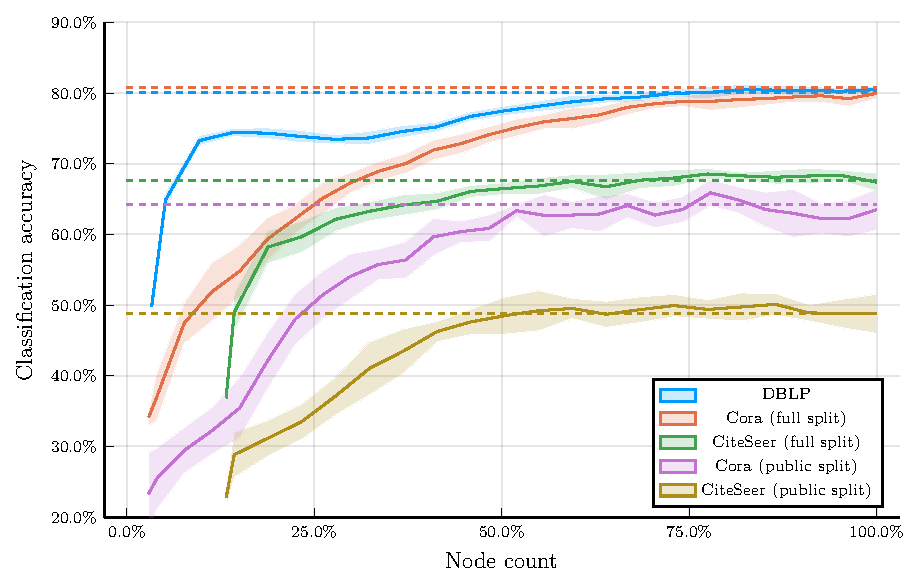
\includegraphics[width = \linewidth]{images/adaptive-coarsening/adaptive-coarsening.pdf}
  \caption{Downstream classifier accuracies at different steps of adaptive prolongation using the basic HARP coarsening algorithm. Dashed line shows the baseline node2vec model accuracy. The node count is taken relative to the total node count in each dataset. The results are averaged over multiple runs, with the solid line representing the mean and the shaded area denoting one standard deviation.}
  \label{fig:adaptive-coarsening}
\end{figure*}

The behaviour of the model somewhat differs between the used datasets. For each dataset, the model starts from a very low performance, which quickly rises as the model trains for several prolongation steps. The model trained on CiteSeer attains performance comparable to the reference model when approximately half of all nodes are available to it. On the other hand, with Cora, the model slowly approaches the reference model for the whole duration of training, only reaching comparable performance at a point where nearly the whole graph is available to it. Models trained on the two larger datasets, DBLP and PubMed, exhibit a substantially different behaviour in that they briefly reach a global maximum followed by a sligh decrease in performance until finally approaching the performance of the reference model in a manner similar to the models trained on Cora and CiteSeer. This behaviour is further dicussed in the next section. The Twitch dataset is substantially different yet again, with very high initial performance and only small performance gains with increasing number of nodes available.

To further study the model properties, the Friedman two-way analysis of ranks was used, with the Holm-Bonferroni correction for multiple hypotheses testing. The hypotheses tested were that the resulting accuracy is the same from the \( k \)-th decile of the node count to the full graph, with tests for all possible values of \( k \). The hypotheses were tested against the 20 testing graphs from the Enzymes dataset, as well as Cora, CiteSeer, DBLP and PubMed. None of the hypotheses were rejected by the test at the 5\% level of significance. We attribute this mainly to the Enzymes dataset, which introduces a lot of noise into the data.

\subsection{The relationship of the results and the properties of the graph}

When the models for DBLP and PubMed are studied more closely, both reach a local maximum at around 14\% of the graph, followed by a slight decline and gradual approach to the baseline. This suggests a global structure in the data, which the model learns at the point of the local maxima. To investigate this hypothesis, several graph metrics were applied to the graphs generated during the adaptive prolongation algorithm run. All of the metrics were applied in two scenarios -- \enquote{absolute}, where the metric was applied to the graph at a particular step in the prolongation process, and \enquote{incremental}, where the metric was applied to the graph induced by the edge set \( \mathspace{C} \), that is, the set of edges to be contracted at that step.

The metrics used were:
\begin{itemize}
  \item Edge homophily \cite{zhu_beyond_2020} is the fraction of edges connecting nodes of the same class.
  \item Node homophily \cite{pei_geom-gcn_2020} is the fraction of node neighbours having the same class as the node in question, averaged over all nodes.
  \item Class homophily \cite{lim_large_2021} is a variant of node homophily that attempts to modify it in such a way as to make it invariant to the number of classes. The metric measures excess node homophily when compared to a null model where edges are independent of node labels.
  \item Adjusted homophily \cite{platonov_characterizing_2022} is a modification of edge homophily targeted at ensuring it is not not biased towards particular class size distributions and that the metric has a constant maximum attained only for perfectly homophilous graphs.
  \item Balanced accuracy \cite{platonov_characterizing_2022} is a modification of edge homophily that balances each classes' contribution.
  \item Adjusted accuracy \cite{platonov_characterizing_2022} is a modification of balanced accuracy aimed at ensuring a constant baseline.
  \item Label informativeness \cite{platonov_characterizing_2022} is a measure of the influence of a node's neighbours' classes to the label of the node itself.
  \item Global assortativity \cite{newman_mixing_2003} is a measure of the tendency of nodes to connect with other similar nodes, rather than dissimilar nodes.
\end{itemize}

The values of these metrics at different steps of the adaptive prolongation algorithm are shown in Figure~\ref{fig:metrics}.

\begin{figure*}
  \centering
  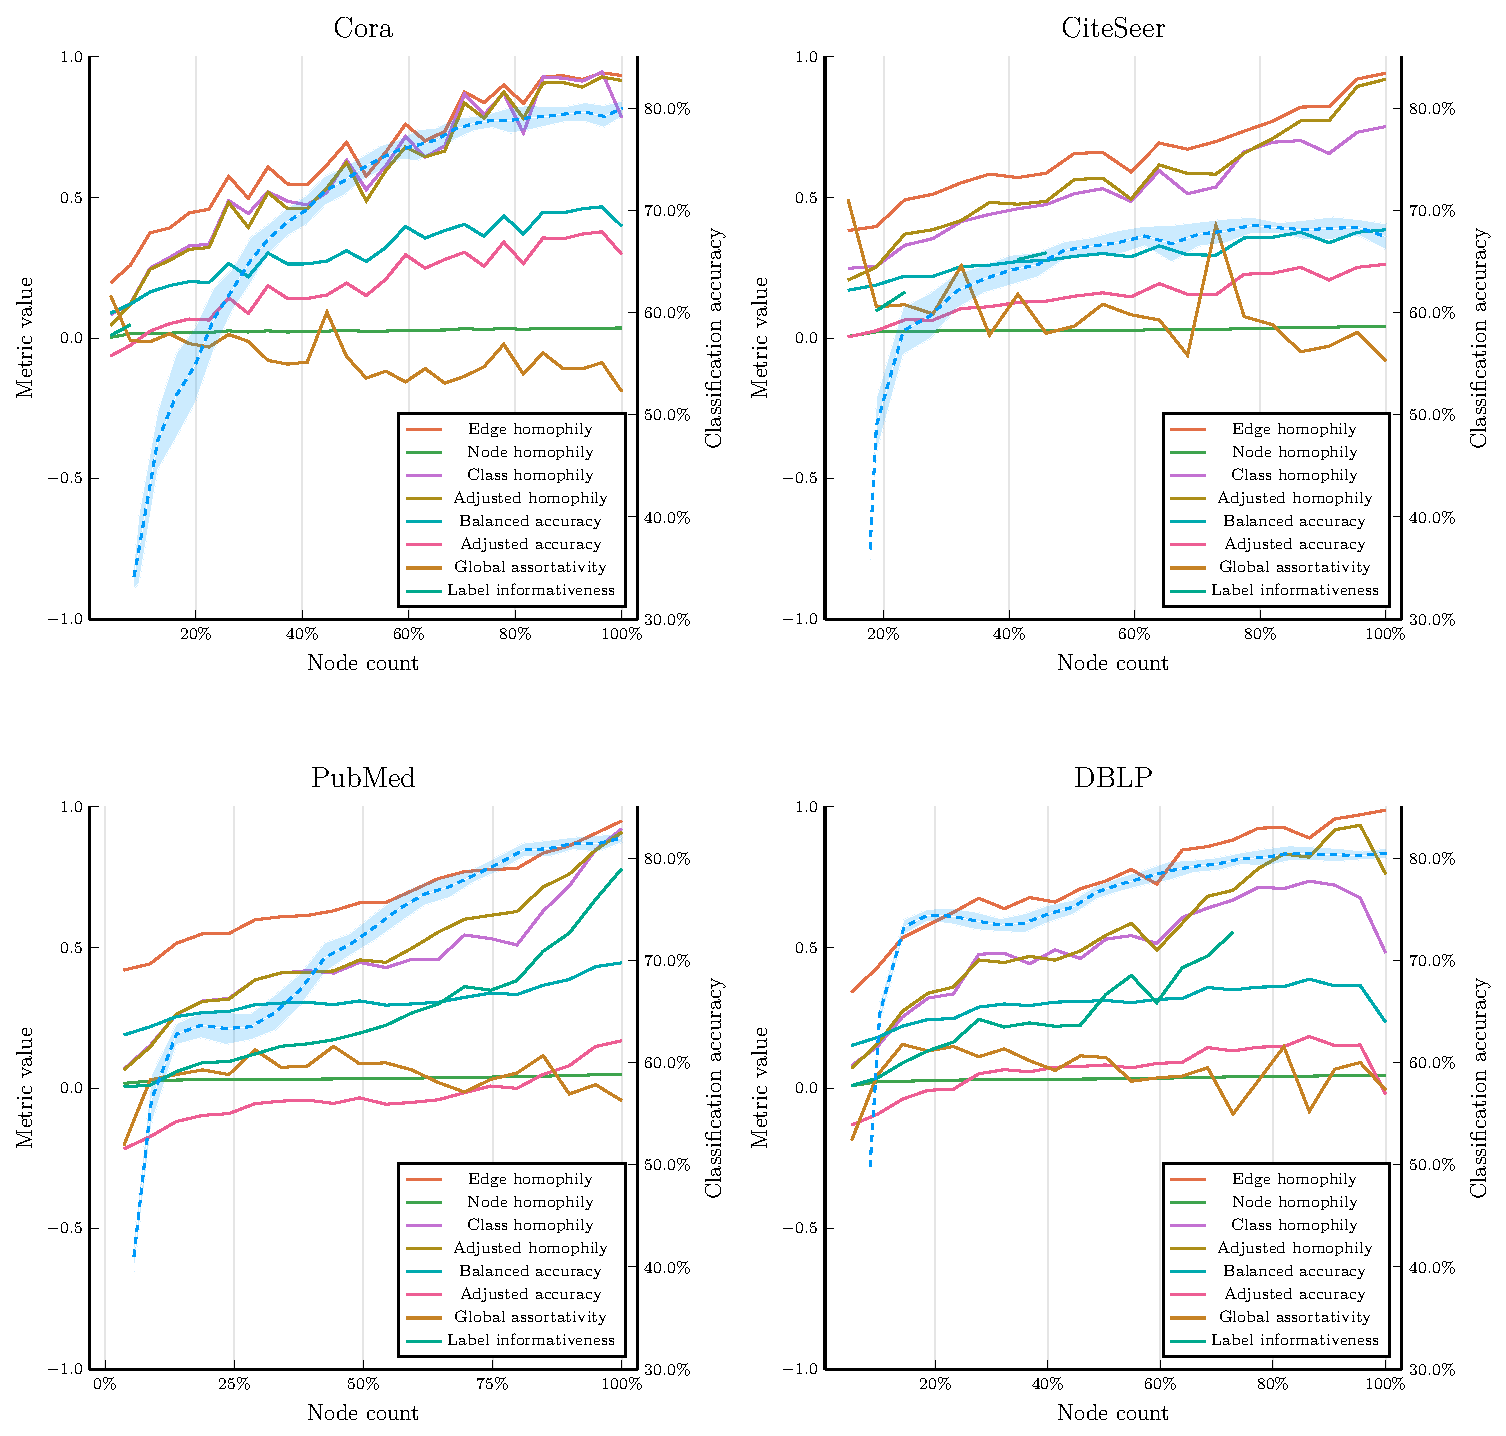
\includegraphics[width = \linewidth]{images/metrics/metrics.pdf}
  \caption{Values of the metrics for different datasets at different steps of the adpative prolongation algorithm. Overlaid as the dashed line is the accuracy of the downstream classifier.}
  \label{fig:metrics}
\end{figure*}

\subsection{Comparison of coarsening approaches}

For GDC coarsening, only the top-\( k \) sparsification method produces reliable results as thresholding leads to instability in the coarsening process, either collapsing the whole graph almost immediately, or not collapsing it at all. As for the other parameters, we followed \cite{gasteiger_diffusion_2019}. Both of the diffusion methods propsed in \cite{gasteiger_diffusion_2019} were implemented with the recommended parameter values, that is the heat kernel was used with the diffusion time \( t = 5 \) and the Personalized PageRank algorithm with the teleport probability \( \alpha = 0.15 \) and the recommended normalization. To be able to compute graph diffusion for larger graphs, approximate diffusion algorithms were used. For PPR, a version of the Andersen algorithm \cite{andersen_local_2006} with \( \epsilon = 10^{-2} \) was used and for heat kernel diffusion, a version of the Kloster-Gleich algorithm \cite{kloster_heat_2014} with \( \epsilon = 10^{-5} \) was used. Both of these algorithms were modified to produce edge weights as part of their output.

For the evolutionary coarsening, the experimental evaluation was conducted with crossover probability \( p_\mathrm{cx} = 0.9 \), individual and gene mutation probabilities \( p_\mathrm{mut} = p_\mathrm{gene} = 0.1 \), parent population size \( \lambda = 3 \), tournament size \( n_\mathrm{tourn} = 3 \), and the individual length \( L \) set to \( 5\% \) of the input graph node count. Each individual was evaluated \( 3 \) times and the results averaged to account for randomness in the evaluation. The set \( \mathspace{AC} \) consisted of 17 atomic coarsenings (Table~\ref{tab:atomic-coarsenings}), where the identity function is limited to maximally be 10\% of the individual. Only four of them had hyper-parameters. These were initialized by random sampling where \( d_\mathrm{lower} \) and \( d_\mathrm{upper} \) were sampled from a Poisson distribution with \( \mu = 30 \) and \( k \) and \( l \) were sampled uniformly from the set of all features. The evolution involved a maximum of 100 generations with an early stopping criterion triggering if the accuracy doesn't change more than 1\% in 10 generations. The evolutionary coarsening algorithm was implemented in the DEAP framework \cite{fortin_deap_2012}.

\begin{table*}
  \begin{center}
    \begin{minipage}{\textwidth}
      \caption{The atomic coarsening functions. In all atomic coarsenings, the edge is selected randomly in case of a tie in the condition.}
      \label{tab:atomic-coarsenings}
      \begin{tabularx}{\textwidth}{Xr}
        \toprule
        \textbf{Set \( \mathcal{C} \) of edges to contract}                                                                     & \textbf{Parameters}    \\
        \midrule
        \( \emptyset \)                                                                                                         &                        \\
        A random edge                                                                                                           &                        \\
        A random edge incident to the highest degree node                                                                       &                        \\
        Edges of a random triangle                                                                                              &                        \\
        The edge whose incident nodes share the highest number of common neighbours                                             &                        \\
        The edge whose incident nodes share the lowest number of common neighbours                                              &                        \\
        A random edge whose incident nodes are adjacent to the highest degree node                                              &                        \\
        A random node of degree at least \( d_\mathrm{lower} \) and its random neighbour                                        & \( d_\mathrm{lower} \) \\
        A random node of degree at most \( d_\mathrm{upper} \) and its random neighbour                                         & \( d_\mathrm{upper} \) \\
        The edge whose incident nodes have the most neighbours in total                                                         &                        \\
        The edge whose incident nodes have the least neighbours in total                                                        &                        \\
        The edge whose incident nodes have the most similar \( k \)-th feature                                                  & \( k \)                \\
        The edge whose incident nodes have the least similar \( l \)-th feature                                                 & \( l \)                \\
        The edge whose incident nodes have the most similar features under the \( L^2 \) distance                               &                        \\
        The edge whose incident nodes have the least similar features under the \( L^2 \) distance                              &                        \\
        The edge whose incident nodes have the most similar set of features of 1-hop neighbours (under the Hausdorff distance)  &                        \\
        The edge whose incident nodes have the least similar set of features of 1-hop neighbours (under the Hausdorff distance) &                        \\
        \bottomrule
      \end{tabularx}
    \end{minipage}
  \end{center}
\end{table*}

\begin{figure*}
  \centering
  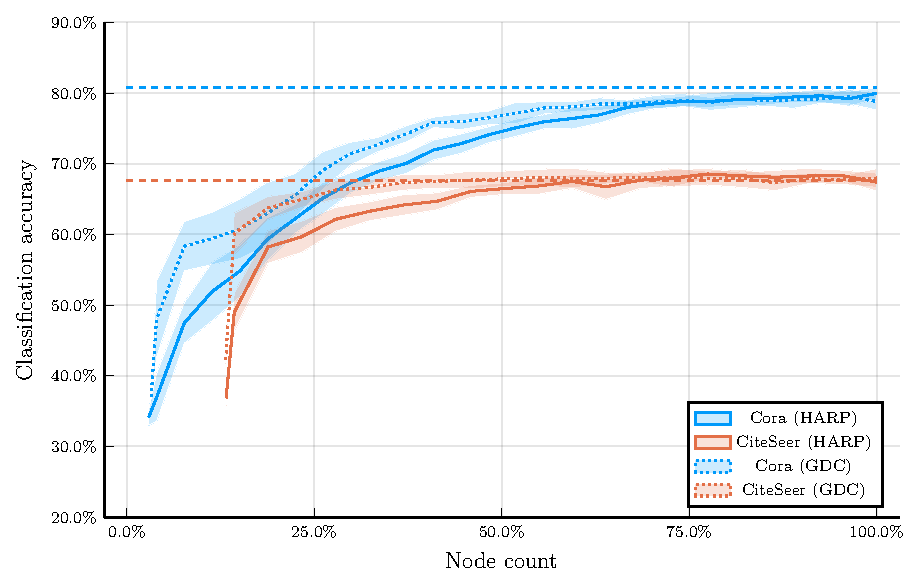
\includegraphics[width=\linewidth]{images/coarsening-algorithms/coarsening-algorithms.pdf}
  \caption{Downstream classifier accuracies at different steps of adaptive prolongation for different coarsening algorithms. Dashed line shows the baseline node2vec model accuracy. The node count is taken relative to the total node count in each dataset. The results are averaged over multiple runs, with the solid line representing the mean and the shaded area denoting one standard deviation.}
  \label{fig:coarsening-algorithms}
\end{figure*}

The behaviour of the models (Figure~\ref{fig:coarsening-algorithms}) again differs substantially between the datasets. As in the previous experiment, the Enzymes dataset contains a lot of noise and generally, the methods behave in a similar manner, retaining decent performance even at the coarsest levels and only improving slightly as more data is available. For both the Cora and the CiteSeer dataset, a clear trend emerges where the GDC coarsening quickly outperforms the original HARP coarsening, with PPR producing better results on Cora under heavy coarsening and both having similar behaviour on CiteSeer. The larger portions of the data the algorithms see, the more the margin shrinks until it vanishes completely. This suggests that the GDC algorithm is able to better preserve the global structure of the graph over successive coarsenings. On the other hand, the evolved coarsening clearly performs the worst, being outperformed by all other methods.

An identical statistical test to the one described in Section~\ref{sec:adaptive-experiments} was carried out for all of the coarsening algorithms. Only the GDC coarsening with the heat kernel rejected the hypothesis that the accuracy is the same from the \( k \)-th decile onwards at the 5\% significance level, for \( k \in \left\{ 1, 2, 3 \right\} \). The Holm-corrected familywise p-values for \( k \in \left\{ 1, 2, 3, 4, 5 \right\} \) were \( 0.019, 0.023, 0.027, 0.071, 0.8 \), respectively. For other algorithms, the hypotheses weren't rejected for any value of \( k \).

\section{Conclusion}

In our work in progress, a way to merge method generality, computational efficiency and high performance was explored. HARP and partially injective homomorphisms were presented and subsequently connected as a way to, in a future work, adapt graph coarsenings to a specific task. This connection was experimentally verified not to impact prediction performance. Furthermore, the effect of HARP pretraining on learning characteristics was studied and found to reduce the need for training on fine (and therefore large) graphs, making way for a more efficient training without sacrificing performance.


\begin{acknowledgments}
  The research reported in this paper has been supported by the German Research Foundation (DFG) funded project 467401796.
\end{acknowledgments}

\bibliography{zotero}

\end{document}
